\section{定点数与浮点数}\label{sec:NumberSystemBasics/FixedPointAndFloatingPoint}
    解决了整数的二进制记录问题之后,我们需要考虑小数的记录的问题。

    我们可以参考在整数时使用的方式,直接记录小数的二进制,但是这会造成一个问题:由于二进制只有两个可用的记号 $0$ 和 $1$,而且它们都已经被用来表达数字,因此已经没有记号可以用来在数码之间标记出小数点的位置且不造成歧义。显然,“小数点在哪里”这个问题有两种解决方案,一种是事先约定好小数点的位置,一种是划出一段空间用来记录小数点的位置。

    \subsection{定点数}\label{subsec:NumberSystemBasics/FixedPointAndFloatingPoint/FixedPoint}
        对于一个有 $k$ 位的设备,如果我们事先约定小数点的位置在 $n$ 位与 $n + 1$ 位之间的话,那么这个小数的表达方式就能总结为如下几点:
        \begin{enumerate}
            \item 左起第一位为符号位;
            \item 左起第二位到第 $n$ 位是整数部分的二进制记录;
            \item 左起第 $n + 1$ 位到第 $k$ 位是小数部分的二进制记录。
        \end{enumerate}

        此时它可以表达的数的范围是 $(-\underbrace{11 \cdots 11}_{n-1}.\underbrace{11 \cdots 11}_{k-n})_2$ -- $(-0.\underbrace{00 \cdots 00}_{k-n}1)_2$ 和 $(0.\underbrace{00 \cdots 00}_{k-n}1)_2$ -- $(\underbrace{11 \cdots 11}_{n-1}.\underbrace{11 \cdots 11}_{k-n})_2$,或者说 $-\frac{2^{(k-1)}-1}{2^{(k-n)}}$ -- $-\frac{1}{2^{(k-n)}}$ 和 $\frac{1}{2^{(k-n)}}$ -- $\frac{2^{(k-1)}-1}{2^{(k-n)}}$,分度值为 $(0.\underbrace{00 \cdots 00}_{k-n}1)_2$,或者说 $\frac{1}{2^{(k-n)}}$。

        一个具体的例子如~\ref{fig:NumberSystemBasics/FixedPointAndFloatingPoint/FixedPoint/DataRange} 所示。

        % https://tex.stackexchange.com/a/130008/149813
        \begin{figure}
            \centering
            \begin{tabular}{lS[table-format=-3.7]S[table-format=-3.7]S[table-format=-3.7]}
                $n$ & 最小值     & 最大值    & 分度值    \\ \hline
                1   & -0.9921875 & 0.9921875  & 0.0078125 \\
                2   & -1.984375  & 1.984375   & 0.015625  \\
                3   & -3.96875   & 3.96875    & 0.03125   \\
                4   & -7.9375    & 7.9375     & 0.0625    \\
                5   & -15.875    & 15.875     & 0.125     \\
                6   & -31.75     & 31.75      & 0.25      \\
                7   & -63.5      & 63.5       & 0.5       \\
                8   & -127       & 127        & 1         \\
            \end{tabular}
            \caption{$k = 8$ 时 $n$ 的值对应的数据范围}
            \label{fig:NumberSystemBasics/FixedPointAndFloatingPoint/FixedPoint/DataRange}
        \end{figure}

        对于以上的定义,

        这种记录小数的方式,在一开始小数点的位置就被固定了,因此称为“定点数”(Fixed Point):比如说,对于二进制小数 $(100.11)_2$ 来说,不管如何修改 $k$ 和 $n$,这个数的小数点的位置总是在第二个 $0$ 和第二个 $1$ 之间,这个小数点的位置是固定不变的,这就是“定点数”一名的来源。

        然而,这种记录方式有一个问题:精度与范围只能二选一。如果使用更小的 $n$,精度就能提高,但是所能表达的数的范围便急剧减小;如果提升表达的数的范围,就需要使用更大的 $n$,这导致了精度的降低。如果我们将所使用的权重画出来,就会是如图~\ref{fig:NumberSystemBasics/FixedPointAndFloatingPoint/FixedPoint/Position} 所示的情况:

        \begin{figure}
            \centering
            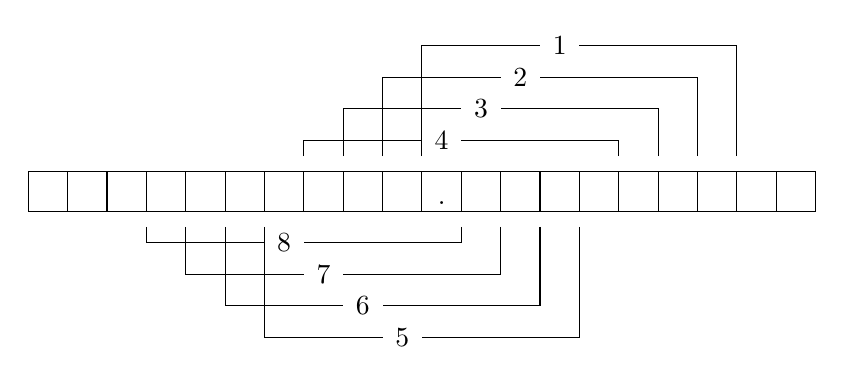
\begin{tikzpicture}
                \draw [step = 0.5] (0, 0) grid (10, 0.5);
                \node at (5.25, 0.1) {.};

                \draw (1.5, -0.2) -- (1.5, -0.4) -- (3, -0.4);
                \draw (5.5, -0.2) -- (5.5, -0.4) -- (3.5, -0.4);
                \node at (3.25, -0.4) {8};

                \draw (2, -0.2) -- (2, -0.8) -- (3.5, -0.8);
                \draw (6, -0.2) -- (6, -0.8) -- (4, -0.8);
                \node at (3.75, -0.8) {7};

                \draw (2.5, -0.2) -- (2.5, -1.2) -- (4, -1.2);
                \draw (6.5, -0.2) -- (6.5, -1.2) -- (4.5, -1.2);
                \node at (4.25, -1.2) {6};

                \draw (3, -0.2) -- (3, -1.6) -- (4.5, -1.6);
                \draw (7, -0.2) -- (7, -1.6) -- (5, -1.6);
                \node at (4.75, -1.6) {5};

                \draw (3.5, 0.7) -- (3.5, 0.9) -- (5, 0.9);
                \draw (7.5, 0.7) -- (7.5, 0.9) -- (5.5, 0.9);
                \node at (5.25, 0.9) {4};

                \draw (4, 0.7) -- (4, 1.3) -- (5.5, 1.3);
                \draw (8, 0.7) -- (8, 1.3) -- (6, 1.3);
                \node at (5.75, 1.3) {3};

                \draw (4.5, 0.7) -- (4.5, 1.7) -- (6, 1.7);
                \draw (8.5, 0.7) -- (8.5, 1.7) -- (6.5, 1.7);
                \node at (6.25, 1.7) {2};

                \draw (5, 0.7) -- (5, 2.1) -- (6.5, 2.1);
                \draw (9, 0.7) -- (9, 2.1) -- (7, 2.1);
                \node at (6.75, 2.1) {1};
            \end{tikzpicture}
            \caption{存储位的位置}
            \label{fig:NumberSystemBasics/FixedPointAndFloatingPoint/FixedPoint/Position}
        \end{figure}
